% !TeX root = ../main.tex
% Add the above to each chapter to make compiling the PDF easier in some editors.

\chapter{Introduction}\label{chapter:introduction}

The Zipfian distribution is a power law that has been observed in a wide range of natural and artificial phenomena. 
It is characterized by the fact that the frequency of an element is inversely proportional to its rank, meaning the position of the element in the sorted list of elements.
A quick example makes this principle quite clear.

\begin{figure}[ht!]
  \centering
  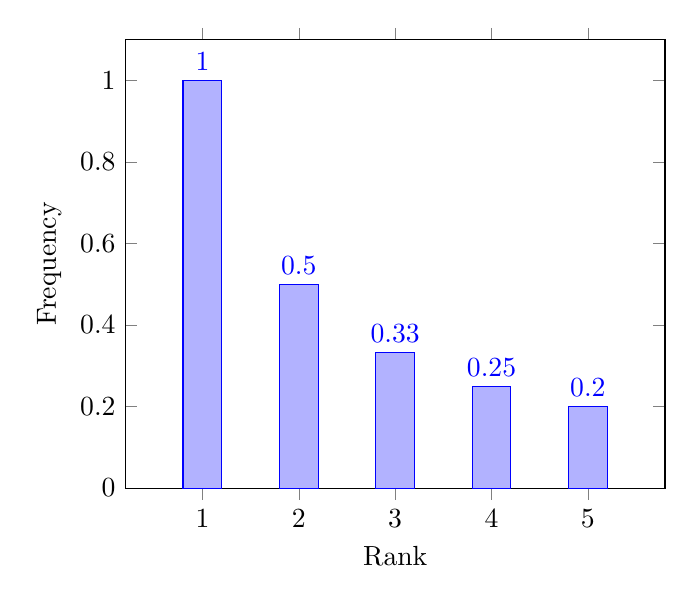
\begin{tikzpicture}
  \begin{axis}[
    ybar,
    bar width=14pt,
    enlarge x limits=0.2,
    symbolic x coords={1,2,3,4,5},
    xtick=data,
    xlabel={Rank},
    ylabel={Frequency},
    ymin=0, ymax=1.1,
    nodes near coords,
    ]
    \addplot coordinates {
      (1,1)     
      (2,0.5)   
      (3,0.333) 
      (4,0.25)   
      (5,0.2)    
    };
  \end{axis}
\end{tikzpicture}

  \caption{Example of a Zipfian distribution}
  \label{fig:zipf_example} 
\end{figure}

This means that the most frequent element is twice as frequent as the second most frequent element, three times as frequent as the third most frequent element, and so on. 
This distribution has been observed in a wide range of natural phenomena, such as the distribution of words in natural languages, the distribution of cities by population, among others \cite{mandelbrotNatureFractal1998}. And also within the fields of storage systems research, networking theory
as well as databases, there has been more compelling evidence that the Zipfian distribution (or more generally, heavy-tailed distributions) is a good model for the distribution of access patterns in these systems \cite{grayQuicklyGeneratingBillionrecord1994, crovellaPerformanceEvaluationHeavy2000,deanTailScale2013}.

The focus however of this thesis is on the large-scale generation of Zipfian samples, which are essential for the evaluation of latency and general performance in storage systems and databases. 
To this end, the state-of-the-art in synthetic workload generation is reviewed and common solutions are identified and evaluated. Parallely, a study of variate generation algorithms is conducted, with a focus on the generation of Zipfian variates.
This will allow for the comparison in terms of speed and accuracy of common implementations as well as give a baseline for an improved version. The main contributions of this thesis are:
\begin{itemize}
  \item A review of the state-of-the-art in synthetic workload generation, with a focus on the generation of Zipfian variates.
  \item A study of variate generation algorithms, with a focus on the generation of Zipfian variates.
  \item An implementation of a Zipfian variate generator in C++20, with a focus on performance and algorithmic simplicity
  \item An evaluation of the performance of the implemented Zipfian variate generator in comparison to existing solutions
\end{itemize}

The results show that existing solutions are generally accurate and fast, while one framework, FIO, is incorrect for larger sample sizes. One of the algorithms, \textit{Rejection-Inversion}, 
is still one of the fastest and the most accurate for generating variates of the target distribution, though table methods could present a new alternative if further optimized. Generally
implementations based in Java, with around $27$ million variates per second, were between $1.4$ and $1.8$ times slower than their C/C++ counterparts, with around $44$ million variates per second. 
As such, these implementations can still be recommended for synthetic workload generation. Furthermore accuracy analysis shows that the implementations found
in common benchmark suites are quite accurate: the ratio between sampled frequencies and theoretical ones are quite close to $1$ for sampel sizes $10$ times the support size while maximal
absolute error is around $10^{-3}$. It was also found out that the sampled distributions converge quite fast, with $10$ times the sample size being a good rule of thumb for the number of samples needed.
